\chapter{Convolution Neural Network Model}
\label{chap:cnn}

\section{Architecture}
For VMMR tasks, a simple Convolution Neural Network (CNN) model is also considered, as presented in \ref{fig:cnn}.

\begin{figure}
\centering
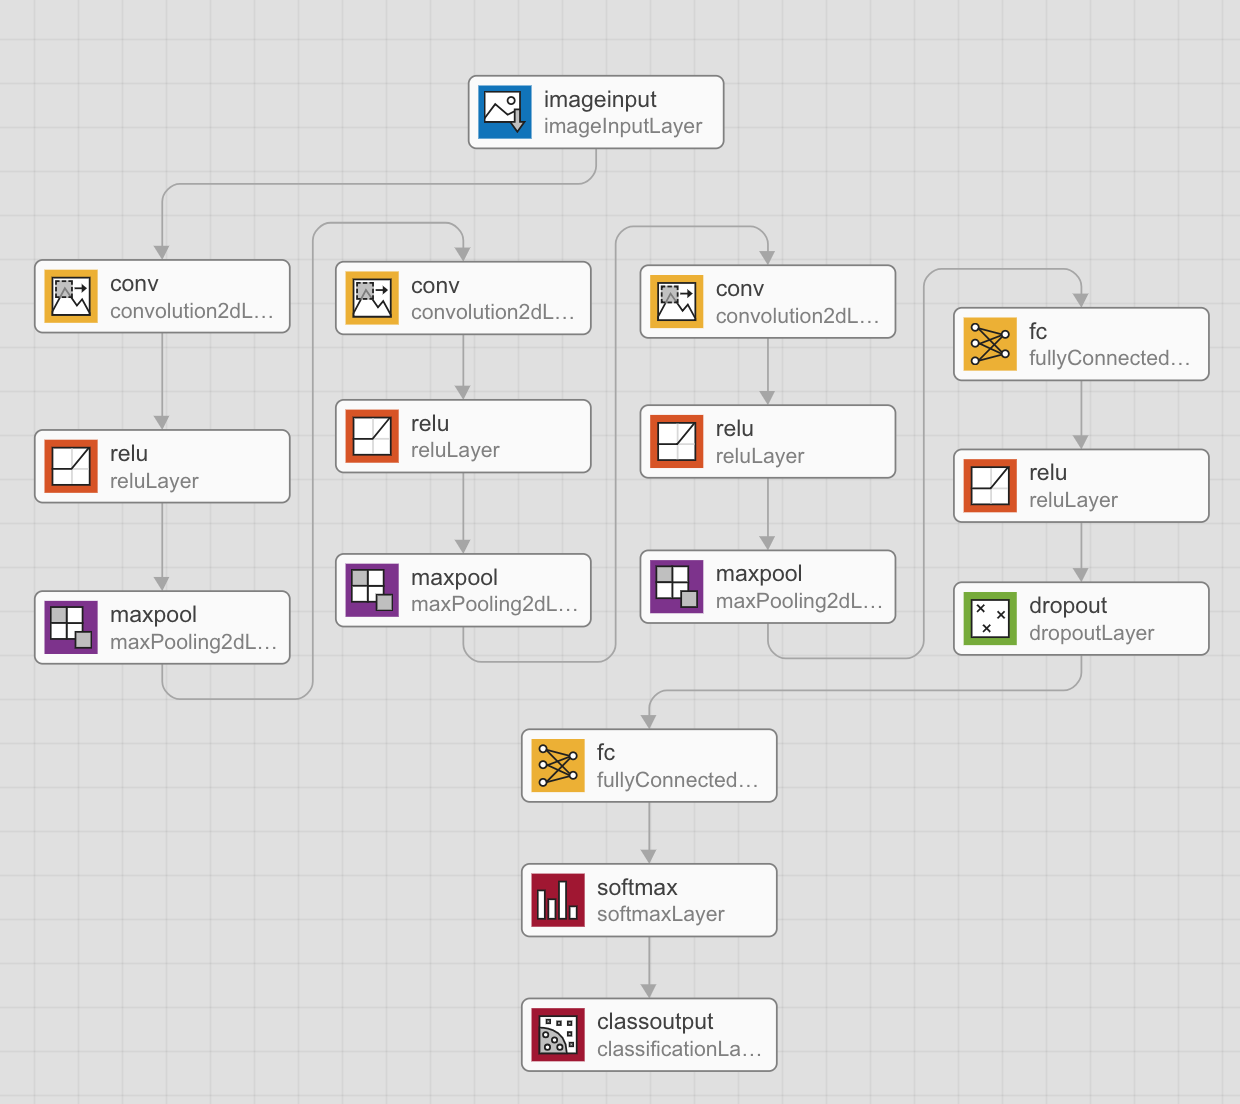
\includegraphics{cnn}
\caption{Architecture of Our Proposed CNN.}
\label{fig:cnn}
\end{figure}

The input image of size $(140, 140, 1)$ is fed into the first convolution layer and activated by a ReLU function. The convolution layer has $32$ filters of $(5, 5)$, stride of $2$ and produces an output of $(70, 70, 32)$.
The layer picks up simple features such as edges, colours, curves from the image.
It is followed by a max pooling layer with filter size of $(3, 3)$ and stride of $2$ to reduce dimensionality. The output has a size of $(35, 35, 32)$ and is fed into the second convolution layer.

The second convolution layer has $32$ filters of $(3, 3)$, stride of $2$ and produces an output of $(18, 18, 32)$. 
The layer picks up more specific features such as squares, circles and triangles from the image.
It is activated by a ReLU function and followed by a max pooling layer with filter size of $(3, 3)$ and stride of $2$ to reduce dimensionality. The output has a size of $(9, 9, 32)$ and is fed into the third convolution layer.

The third convolution layer also has $32$ filters of $(3, 3)$, stride of $1$ and produces an output of $(9, 9, 32)$. 
This layer picks up high-level features such as headlights, front beams, logos from the image.
It is activated by a ReLU function and followed by a max pooling layer with filter size of $(3, 3)$ and stride of $2$ to reduce dimensionality. The output has a size of $(5, 5, 32)$ and is fed into the first fully connected layer.

The first fully connected layer has $256$ hidden units and is activated by a ReLU function. This layer introduces more complexity into the network and allows high-level features located at different locations in the image to be combined.
It is followed by a dropout layer with rate of $0.5$, which introduces regularization into the model and prevents over-fitting.
The output is fed into the second fully connected layer.

The first fully connected layer has $27$ hidden units, the same size as the number of vehicle classes, and is activated by a Softmax function for the final classification output.


\section{Overfitting Issues}
Our proposed CNN model has $213,467$ parameters, much larger to other machine learning models used previously. Thus, the model is prune to overfitting.
The following strategies can be adopted to prevent overfitting in the model.

\begin{enumerate}
\item
	Introduce a regularization term into the loss function. That is, the new loss function $L_{new}(W) = L(W) + \lambda R(W)$, where $R(W)$ is a regularization term for the weights $W$. Typically, $R(W) = W^2$ and it forces the network to make full use of the inputs at each layer.
\item
	Introduce a dropout layer in between different layers. The dropout layer randomly drops a percentage of its input, thus forcing the next layer to not rely on a small set of its inputs.
\item
	Early stopping. When the model is being trained on the dataset, the decrease in loss on the training set and the increase in loss on the validation set is a sign of overfitting. In such cases, the model should be stopped training to prevent further overfitting.
\end{enumerate}

\section{Insufficient Dataset}
Given the small size of our dataset ($530$ images in total), the average number of parameters per image is $403$. 
Such amount of paramters signal that the size of our dataset is insufficient.
In the case that time and resouces are limited for collecting new data, several alternative solutions could be considered.

\begin{enumerate}
\item
	Apply data augmentation to the dataset to generate more images for training. The operations for data augmentation include rotation, scaling, shearing and translation.
\item
	Use pre-trained CNN models such as AlexNet\citep{krizhevsky2012imagenet}, GoogLeNet\cite{szegedy2015going} and ResNet\citep{he2016deep} in a transfer learning scheme. Since our dataset is small, it is difficult to fine-tune the whole network. Therefore, only the last few layers of pre-trained CNN networks are replaced and re-trained.
\end{enumerate}


% \section{Performance}






